\begin{figure}[ht]
\centering
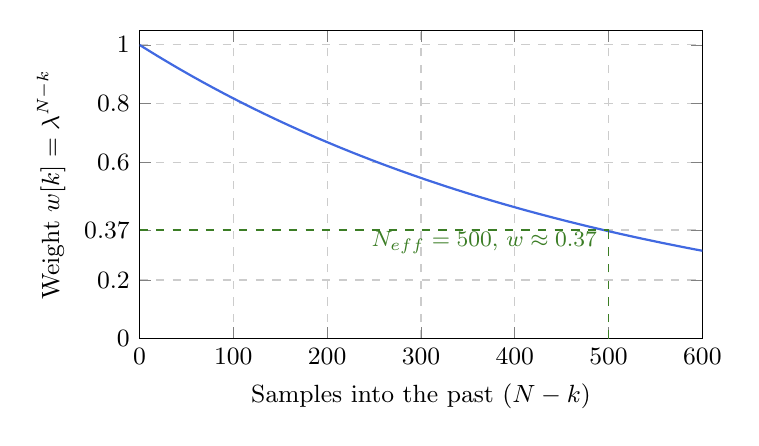
\begin{tikzpicture}
\begin{axis}[
  width=0.72\textwidth, height=5.5cm,
  xlabel={Samples into the past ($N-k$)},
  ylabel={Weight $w[k]=\lambda^{N-k}$},
  xmin=0, xmax=600, ymin=0, ymax=1.05,
  xtick={0,100,200,300,400,500,600},
  ytick={0,0.2,0.37,0.6,0.8,1.0},
  grid=major, grid style={dashed,gray!40},
  tick label style={font=\small}, label style={font=\small},
]
\addplot[thick, RoyalBlue, domain=0:600, samples=150] {0.998^x};
\addplot[dashed, OliveGreen, domain=0:500] {0.37};
\addplot[dashed, OliveGreen] coordinates {(500,0) (500,0.37)};
\node[font=\footnotesize, OliveGreen, anchor=north east]
  at (axis cs:498,0.40) {$N_{eff}=500$, $w\approx 0.37$};
\end{axis}
\end{tikzpicture}
\caption{Exponential weight decay with $\lambda=0.998$.
  Data older than $N_{eff}=1/(1-\lambda)=500$ samples has weight $\leq e^{-1}\approx 0.37$.}
\label{fig:forgetting-factor}
\end{figure}
